\chapter{OpenBTS with a cognitive approach}


\section{Target}

Our goal is to set up an OpenBTS system with cognitive capabilities. We decide on a frequency channel, to run our cognitive OpenBTS system in, beforehand. First we sense the presence of ongoing calls made by primary users in the predefined frequency channel. If there are ongoing calls in that channel then we wait for the calls to end. As soon as the calls made by primary users end, we start our secondary OpenBTS system to allow secondary users to make calls.

\section{Spectrum Sensing}

Spectrum sensing is the task of finding spectrum holes (or empty spectrum) in the local neighborhood of the cognitive radio receiver. Spectrum holes are the empty or unused portions of the spectrum at a particular space and time. Spectrum sensing lies at the very heart of cognitive radio technology. Cognitive radio works by utilizing the unused portions of the spectrum and for this to be possible, we need to find those empty portions of the spectrum at the very first. 

Detecting the presence of primary users is considered the most efficient way of spectrum sensing. Some of the ways to detect primary users are:

\begin{itemize}
	\item Energy detection
	\item Matched filter detection
	\item Cyclostationary detection
\end{itemize}

\subsection{Energy Detection}

This method of detecting primary users is the simplest one. It requires no a-priori knowledge about the signal to be detected. Basically the energy of the frequency band in question is calculated and compared to a predefined threshold to determine whether a primary user is present in that frequency band or not. Energy detection is simple to implement and relatively not so expensive in terms of required computing resources.
This method is not without disadvantages. Firstly deciding on a good threshold energy level is difficult. It cannot differentiate between primary users and secondary users. At low SNR, distinguishing a signal from noise is difficult. Averaging out the noise by using longer observation period can also lead to inefficient use of time. 

\begin{figure}[h]
\centering
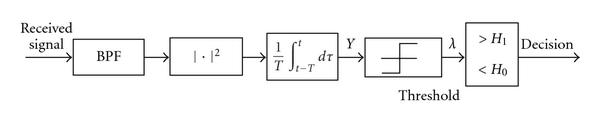
\includegraphics[width=1\textwidth]{energyDetector}
\caption[Block diagram of Energy Detection implementatio]{Block diagram of Energy Detection implementation. \emph{Source: \url{http://www.hindawi.com/journals/ijvt/2011/630467.fig.003.jpg} [Accessed on Oct 22, 2013]}}
\label{energyDetector}
\end{figure}




Figure~\ref{energyDetector} gives block diagram to implement the energy detection using the periodogram method.
Spectrum sensing is a binary hypothesis testing problem with tow possible hypothesis $H0$ and $H1$.
The hypothesis $H0$ defines that there is no PU present and hypothesis $H1$ defines that there is a PU present. The goal of energy detection is to distinguish between these two hypothesis \cite{sarijari09}:

\begin{align}
	x(t) &= n(t), \qquad & H0 \nonumber\\
		&= h s(t)+n(t), \qquad & H1 \nonumber
\end{align}

where $x(t)$ is signal received by secondary user and $s(t)$ is signal transmitted by primary user, $n(t)$ is additive white Gaussian noise (AWGN) and $h$ is the amplitude gain of the channel. It is assumed that $s(t)$  and $n(t)$ are independent of each other. Signal detection is performed using an energy detector and compute decision statistics $Y$ which corresponds to energy collected in observation time $Y$ and bandwidth $W$ and comparing this statistics to a predetermined threshold. 

.
\subsubsection{Average Periodogram Analysis}
 It is a technique used as an energy detection method for determining the presence or absence of primary traffic. 
Power spectrum is estimated using periodogram analysis, which is based on discrete fourier 
transform (DFT) of finite length segments of signal. It involves sectioning the data into
finite segments to compute individual periodogram or modified periodogram and averaging the modified periodogram segments \cite{welch67}.


Let $X[n], n=0,1,...,L-$1 be the discrete time signal that are divided into $K$ finite length equal segments,
where length of each segment is $N$ i.e. $KN = L; Xr[n], n= 0,1,..., N-1$ is the $r$th segment and $W[n], n=0,1,...,N-1$ be the window applied to each segment. The modified periodogram for the $r$th segment is,

\begin{equation*}
	I_{r}[k] = \frac{1}{NU}\vert{}V_{r}[k]\vert{}^2     \qquad k=0,1,...,N-1
\end{equation*}

where $V_{r}[k]$ is a $N$ point DFT and $U$ is normalization factor i.e. ,
$V_{r}[k] = DFT\{W[n]*X[n]\}$  and 
$U = \frac{1}{N}(\sum_{n=0}^{N-1}(W[n])^2)$.


The PSD of $X[n]$ sequence or the time averaged periodogram estimate ,
\begin{equation*}
\bar{I}[k] = \frac{1}{K}\sum_{r=0}^{K-1}Ir[k]
\end{equation*}

One of the most relevant tools for wide band spectrum sensing is GNU radio spectrum sensor \mbox{``usrp\_spectrum\_sense.py''.}
 This program can be used as a basic code for implementing wideband spectrum analyzer. The output is  $Y[i] = re[X[i]]*re[X[i]] + im[X[i]]*im[X[i]]$.
To use $N$ point complex FFT $X(W)$ analysis, we have to get $N$ time samples of $x(t)$  which are sampled at $Fs$. These time samples must be time windowed using a known window function to reduce spectral leakage. The output of the complex FFT will represent the frequency spectrum content as follows:
The first value of the FFT output ($bin 0 == X[0]$) is the passband centre frequency
The first half of FFT spectrum ($X[1]$ to $X[N/2-1]$) contains the positive baseband frequencies, which corresponds to the passband spectrum from centre frequency to $+Fs/2$.
The second half of the FFT ($X[N/2]$ to $X[N-1$]) contains the negative baseband frequencies, i.e. from $-Fs/2$ to centre frequency.

In our case, we  gather 1024 samples using a tuner centered at uplink frequency of 900MHz. We chose 1024 as the number of FFT points because the number of FFT points has to be a power of 2 for the fast execution of the FFT algorithm. Sampling frequency is set as 10 MHz by default. The frequency resolution is therefore: 10 MHz / 1024 = 9.7656 MHz.

The \emph{decimation} is defined as \emph{dsp rate} divided by \emph{sample rate}. The UHD driver requires the decimation value to be an even number. The \emph{dsp rate} is the actual hardware-level sampling rate of the USRP kit. It is the rate at which the USRP device takes analog samples from the external world and converts them to digital form.  The \emph{dsp rate} of the USRP is 100MHz. Hence we chose sampling frequency to be 10 MHz which gives a decimation value of: 100 MHz / 10 MHz = 10.

Figure~\ref{workSetup} describes the experimental setup for our project.

\begin{figure}[H]
\centering
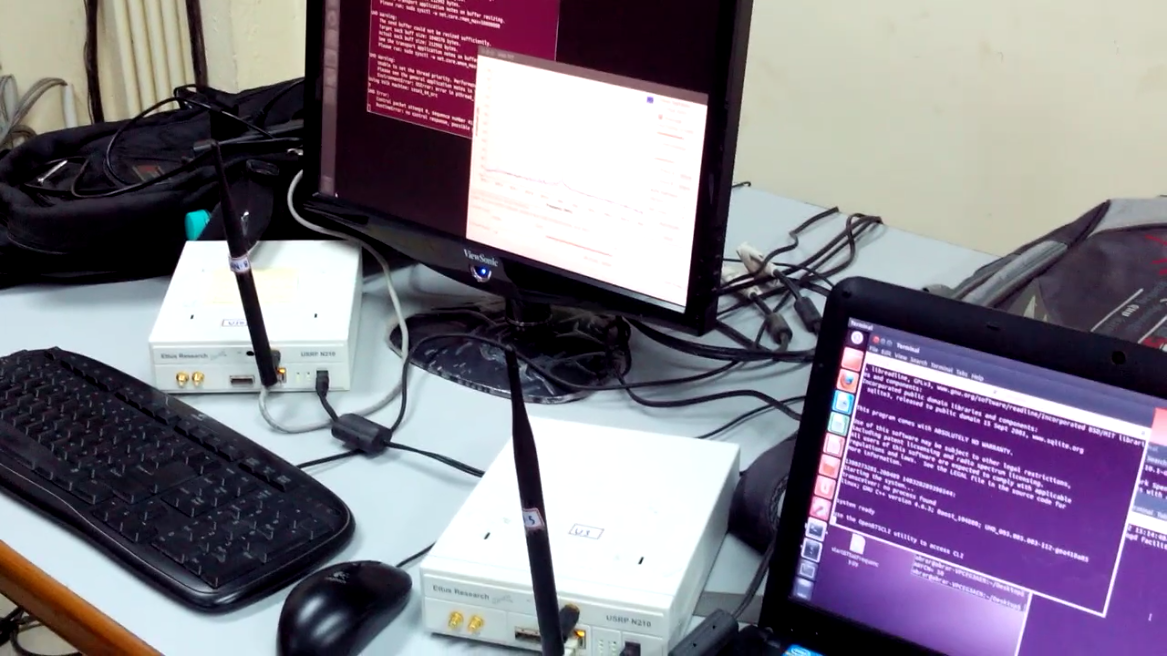
\includegraphics[width=1\textwidth]{workSetup}
\caption[The setup used for the project]{System \textbf{A} is the spectrum analyzer which displays the change in energy when we
initiate a call. System \textbf{B} is the primary OpenBTS and system \textbf{C} is the secondary OpenBTS}
\label{workSetup}
\end{figure}










 
 
We have been able to successfully sense the presence of primary users in the predefined 
frequency band. As soon as the primary user leaves, the energy in that band goes
low and we switch on the secondary BTS and the secondary users are able to make calls and send SMSs using the secondary BTS. 

We have been able to create a python script to kill all the four processes of openBTS. This will be useful in our second stage
work when we might have a loop that starts and kills the OpenBTS as and when it is required. Now, we are also able to run GNURadio and OpenBTS 
on the same computer simultaneously using two USRP kits, one for GNU Radio and the other for OpenBTS. We were not able to do this initially.
GNU Radio will be used to continuously sense the spectrum to detect the presence of primary users and provide the optimum ARFCN for OpenBTS to run in. 

What we aim to achieve is that after GNU Radio has provided the ARFCN corresponding 
to certain frequency (say F1) to OpenBTS, it will continue sensing for primary users in that  
frequency and if it finds that the energy in that
frequency goes above some predefined threshold then secondary OpenBTS will close thus 
avoiding interference to primary users and then it will restart on another frequency(say F2). 
Now GNU Radio will scan for primary users in the frequency F2 and if the energy is found to be above the predefined threshold, then 
the secondary BTS will be turned off and 
restarted on another empty channel. This goes on in a loop again and again.

 
The following flow graph summarizes what we aim to achieve.

\begin{figure}[h]
\centering
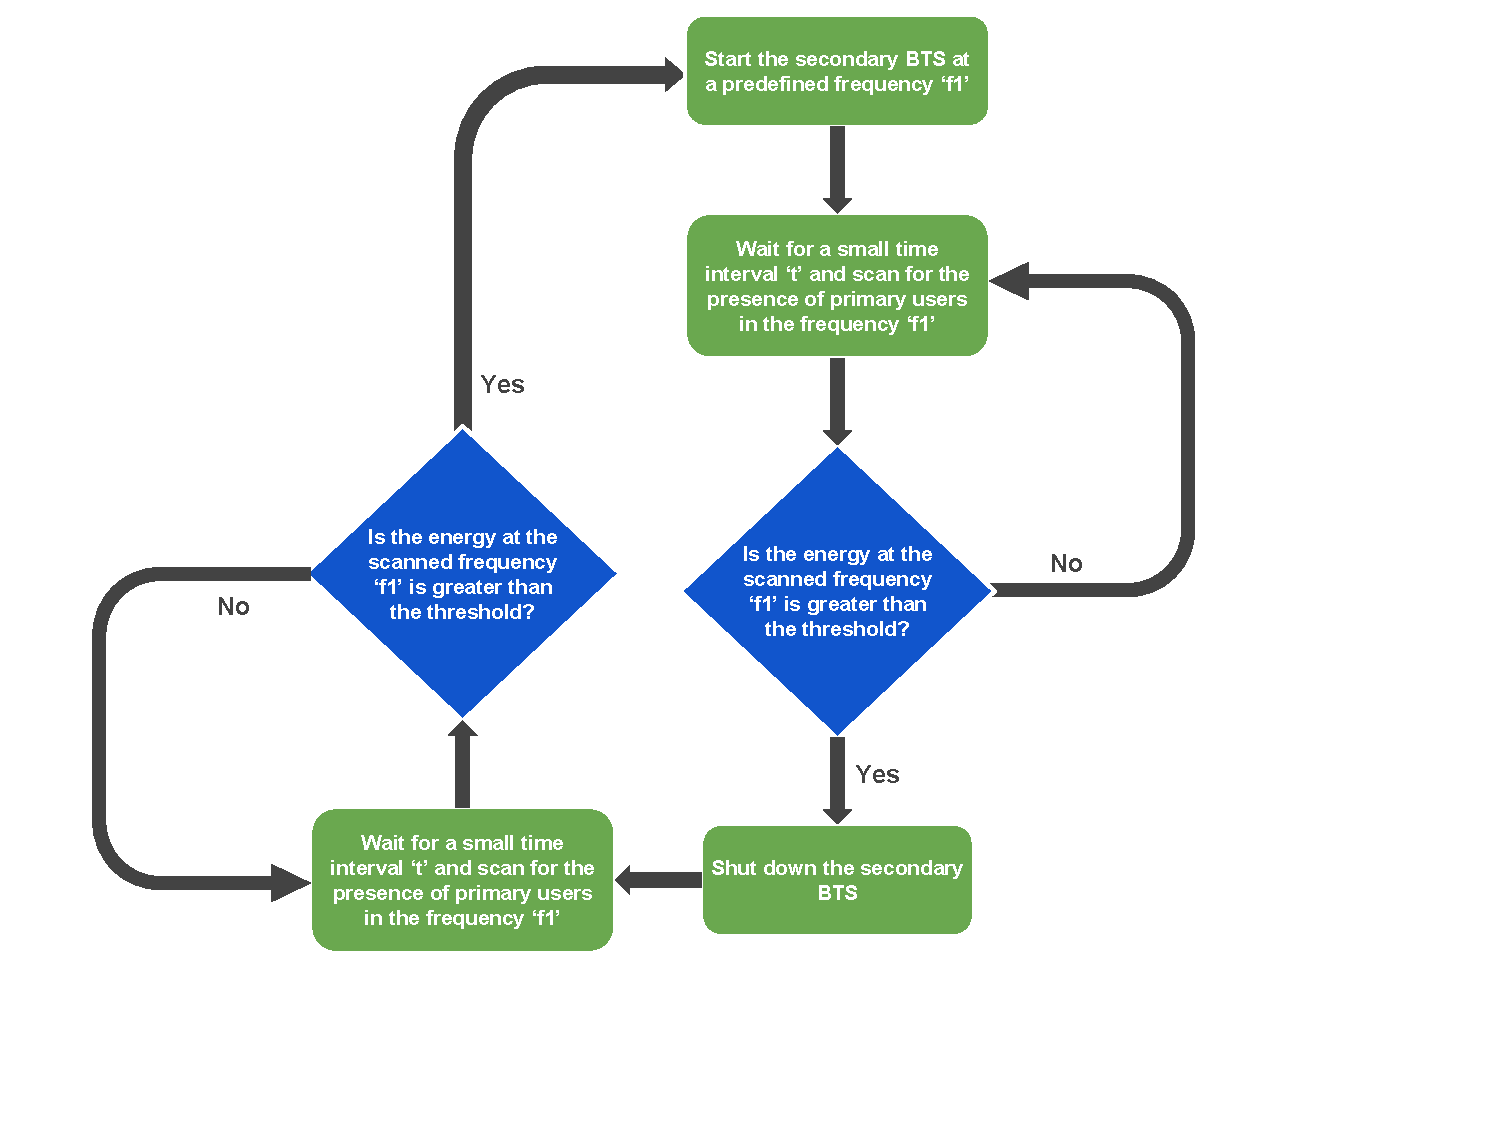
\includegraphics[width=1\textwidth]{workFlowchart}
\caption{Flowchart showing proposed target}
\label{workFlowchart}
\end{figure}

